\section{Estructura de clases}

\subsection{Process Documents}
\begin{frame}{Process Documents}
    Esta clase se encarga de procesar los documentos de la base de datos antes de comenzar la búsqueda.
    Se llama al método en la línea anterior a app.Run () para realizar esta operación una sola vez antes de que
    arranque el programa y esté listo para ejecutarse.

\pause

    \begin{center}
        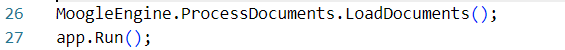
\includegraphics[width=8cm, height=0.75cm]{fig 1.1.png}\\
    \end{center}
\end{frame}  

\subsection{Documents}

\begin{frame}
    \frametitle{Documents}
    Esta clase esta dirigida al trabajo con los documentos, se “normalizan”. Es decir, en caso de que las
búsquedas se realicen en español, se eliminan las tildes para evitar errores ortográficos. Además, independientemente del idioma, se eliminan los signos de puntuación y cualquier otro símbolo ajeno al alfabeto 
y los números.

\pause

\begin{center}
	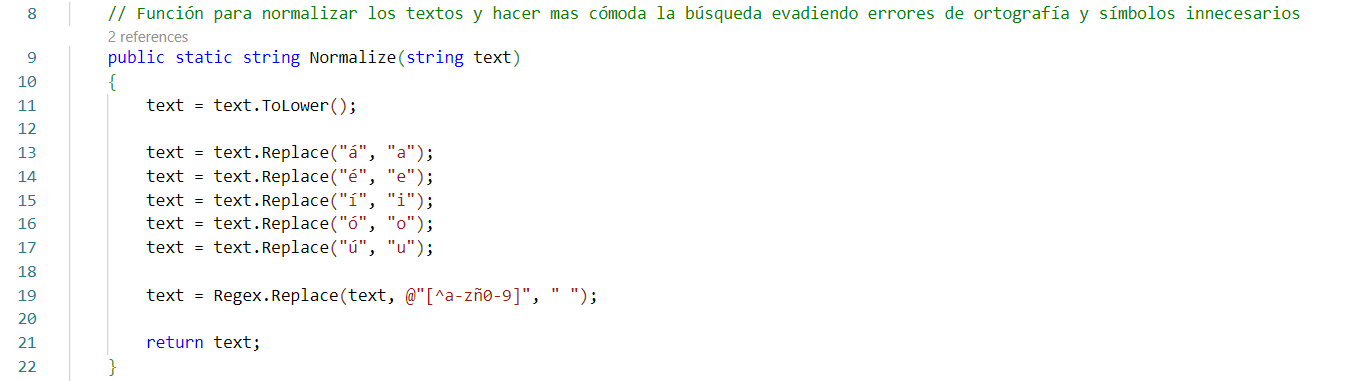
\includegraphics[width=11cm, height=3cm]{fig 1.3.png}\\
\end{center}
\end{frame}

\begin{frame}{Process Documents}
    Se encuentra además esta otra función para seleccionar el “snippet” (pedazo breve de un texto) que se 
    imprimirá en el momento de la búsqueda por cada resultado.

\pause

\begin{center}
	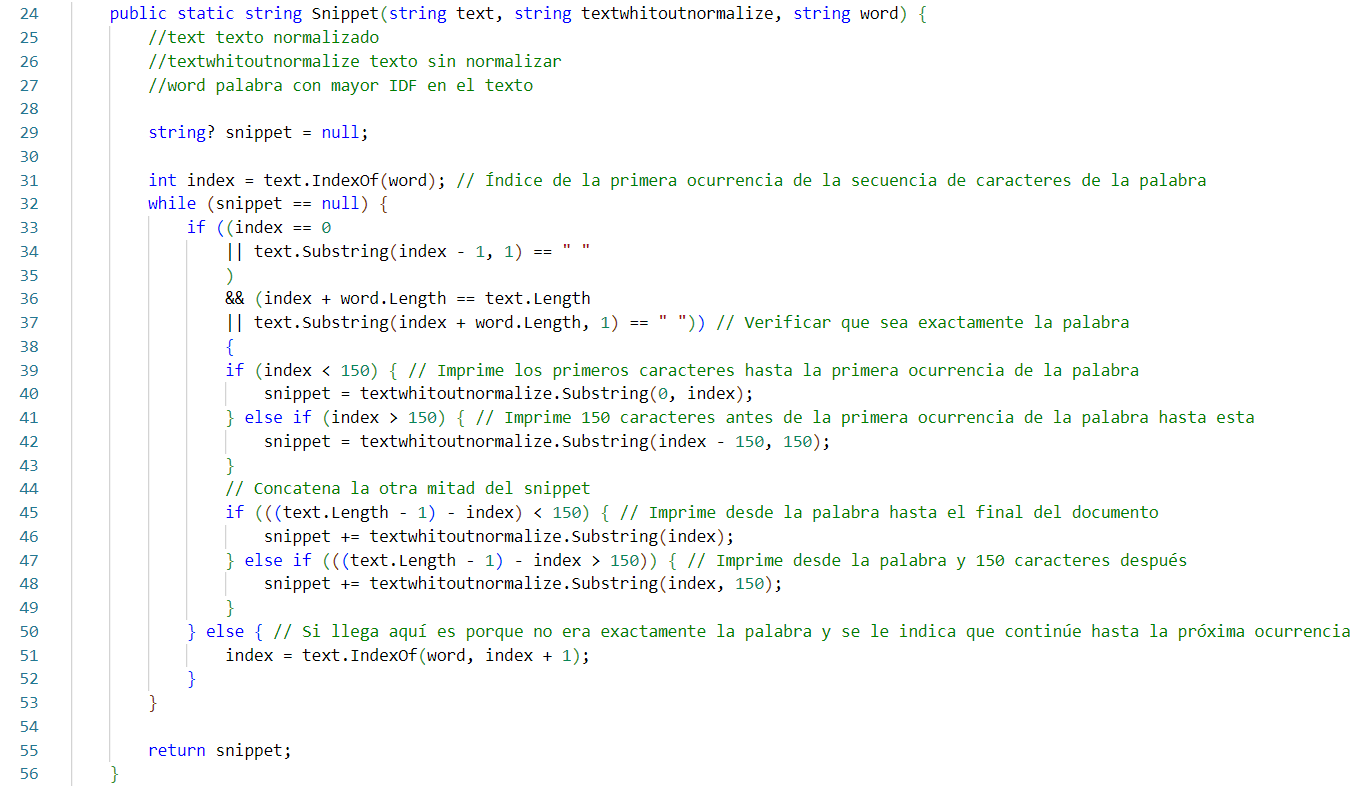
\includegraphics[width=10.7cm, height=5cm]{fig 1.4.png}\\
\end{center}
\end{frame}

\subsection{Matrix}
\begin{frame}{Matrix}
    El valor de “relevancia” de una palabra está dado por el cálculo de su TF (Term Frequency) por su IDF
(Inverse Document Frequency), para ello se ha utilizado la fórmula:

\begin{center}
	$\frac{nd}{Cd} \cdot \log (\frac{T}{N})$ \\
\end{center}

Dónde:
\

\begin{itemize}
    \item nd es la cantidad de ocurrencias de una palabra en un documento,
\pause 
    \item Cd es la cantidad total de palabras en el documento,
\pause
    \item T es la cantidad total de documentos,
\pause
    \item N es la cantidad de documentos en los que aparece la palabra.
\end{itemize}
\end{frame}

\subsection{Moogle}
\begin{frame}{Moogle}
    Esta es la clase principal del programa, donde comienza el proceso de búsqueda. Comienza en el momento
en que se recibe la query.

\pause

\begin{center}
	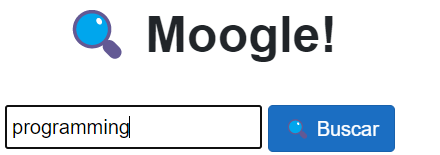
\includegraphics[width=7cm, height=2.7cm]{fig 1.10 (2).png}\\
\end{center}
\end{frame}

\begin{frame}{Moogle}
    Se iteran las palabras sin repetir de la query y se calcula su TF-IDF en los
documentos en los que aparece, pero para conseguir el score por documento se necesita la suma de estos
valores.

\

El score queda de la siguiente manera: si la palabra está contenida en el documento que se está analizando se encontrará el valor de TF-IDF
correspondiente a esa palabra en ese documento, de forma contraria el valor sera 0.

\end{frame}